\documentclass[11pt]{article}
\usepackage[letterpaper,margin=1in]{geometry}
\usepackage{amsmath,amssymb,amsthm}
\usepackage{graphicx}
\usepackage{booktabs}
\usepackage{xcolor}
\usepackage[hidelinks]{hyperref}
\usepackage{enumitem}
\setlist{itemsep=1pt,topsep=3pt}
\usepackage{multicol}
\usepackage[compact]{titlesec}
\titlespacing*{\section}{0pt}{9pt}{4pt}
\titlespacing*{\paragraph}{0pt}{4pt}{0.8em}

\newcommand{\ket}[1]{\lvert #1\rangle}
\newcommand{\bra}[1]{\langle #1\rvert}
\newcommand{\tr}{\operatorname{tr}}
\newcommand{\rank}{\operatorname{rank}}
\newcommand{\one}{\mathbf{1}}
\newcommand{\E}{\mathcal{E}}
\newcommand{\Deph}{\Delta}
% Visible marker for text the group must write or confirm before submitting.
\newcommand{\groupnote}[1]{\textcolor{red}{\textbf{[Group to complete: #1]}}}
\newtheorem{proposition}{Proposition}
\newtheorem{lemma}{Lemma}

\begin{document}
\begin{center}
{\Large\bfseries Quantum Memory for Sequential Prediction:\\[2pt] Classical Limits and the Role of Coherence}\\[6pt]
Alex Tan, Manfredo Ochoa-Aragon, William Noon\\[2pt]
{\small C191A Fall 2026 \textbullet{} Interim report \textbullet{} November 24, 2026}
\end{center}

\begin{abstract}
\noindent To predict a sequence, a model must carry a memory of the past. Hidden Markov models (HMMs) carry a probability distribution; hidden quantum Markov models (HQMMs) carry a quantum state updated by measurements. We ask what quantum coherence in that memory changes, and which comparisons justify calling a quantum model ``more compact.'' So far we have (i)~written HMMs as quantum operations and shown that coherence changes nothing unless the dynamics read it; (ii)~built a one-qubit, four-symbol model that every classical HMM needs at least four states to reproduce, with a lower bound checkable by hand; and (iii)~confirmed that classical HMMs fitted to its data match it at exactly that size. The separation concerns the dimension of a physical memory, not speed, accuracy or parameter count.
\end{abstract}

\section{Introduction and motivation}

Symbols arrive one at a time (words, weather readings, measurement outcomes) and a predictor must keep a summary of what it has seen. How large must that summary be? The question matters wherever memory is costly, and the size of the smallest adequate memory is a natural measure of how complex a process is. Gu \emph{et al.}~\cite{gu2012} showed that quantum systems can simulate some classical random processes with less memory than any classical model, by encoding different pasts into states that are \emph{not} perfectly distinguishable. Ghafari \emph{et al.}~\cite{ghafari2019} demonstrated with photons a qubit doing the work of three classical memory states, and Elliott \emph{et al.}~\cite{elliott2020} found processes where one qubit replaces arbitrarily large classical memories. In parallel, HQMMs, introduced by Monras \emph{et al.}~\cite{monras2010}, were developed in machine learning~\cite{srinivasan2018,adhikary2020} as a model class for sequence data that runs on ordinary computers. Both literatures invite overstatement: ``more compact'' can mean fewer memory dimensions, less memory entropy, fewer parameters, or less computation, and these do not move together. Aaronson's advice for quantum machine learning~\cite{aaronson2015}, read the fine print, applies directly.

\paragraph{Research question.} How does allowing quantum coherence change the representation of a classical random sequence, compared with a classical HMM or a quantum model restricted to diagonal states? \textbf{Q1:} How can HMM dynamics and belief updates be written as quantum operations? \textbf{Q2:} What changes in the sequence distribution when coherence is removed? \textbf{Q3:} Which resource comparisons justify a claim of compactness, and which do not establish a computational advantage?

\paragraph{Expected impact.} A self-contained, checkable account, for a fellow student, of what a ``quantum memory advantage'' for prediction is: a worked example verifiable by hand, a lower bound that certifies the classical side, experiments that test it, and a list of what the advantage does \emph{not} imply. Sections~\ref{sec:embedding}--\ref{sec:resources} contain completed analysis; Section~\ref{sec:plan} lists what remains for the final report (December~4) and poster (December~10).

\section{Background: from hidden Markov models to quantum instruments}\label{sec:background}

\paragraph{Hidden Markov models, from scratch.} Picture a source with a hidden switch in one of $n$ settings. In setting $i$ it prints a symbol $x$ and moves to setting $j$ with probability $T_x[j,i]$, where $\sum_{x,j} T_x[j,i] = 1$. We see only the symbols, so the best we can do is keep a \emph{belief} $b$, a probability vector over the settings. On seeing $x$ it updates by a matrix--vector product and normalisation,
\begin{equation}\label{eq:hmm-update}
  \Pr(x \mid \text{past}) = \one^{\top} T_x b, \qquad b \;\mapsto\; \frac{T_x b}{\one^{\top} T_x b},
\end{equation}
and a whole sequence has probability $\Pr(x_1\cdots x_k) = \one^{\top} T_{x_k}\cdots T_{x_1}\pi$, with $\pi$ the starting belief.

\emph{Example.} Take two settings and symbols $\{0,1\}$. In setting $i$ the source prints $i$ with probability $0.9$, then stays put with probability $0.8$. From the belief $b=(\tfrac12,\tfrac12)$, seeing a $0$ gives $T_0 b = (0.5\cdot0.9\cdot0.8 + 0.5\cdot0.1\cdot0.2,\ 0.5\cdot0.9\cdot0.2 + 0.5\cdot0.1\cdot0.8) = (0.37, 0.13)$. So $\Pr(0) = 0.5$ and the belief becomes $(0.74, 0.26)$. The number of settings $n$ is the classical memory we compare against.

\paragraph{Quantum memory.} In an HQMM the memory is a $d$-dimensional quantum system in state $\rho$. Producing a symbol is a measurement: the memory interacts with a fresh ancilla through a unitary and the ancilla is measured. Outcome $x$ then acts on the memory as
\begin{equation}\label{eq:instrument}
  \E_x(\rho) = \sum_{w} K_{x,w}\,\rho\,K_{x,w}^{\dagger}, \qquad \sum_{x,w} K_{x,w}^{\dagger}K_{x,w} = I,
\end{equation}
with Kraus operators $K_{x,w}$; completeness makes the probabilities sum to one, and $\{\E_x\}$ is called a quantum instrument. Prediction and update mirror Eq.~\eqref{eq:hmm-update}:
\begin{equation}\label{eq:hqmm-update}
  \Pr(x\mid\text{past}) = \tr \E_x(\rho), \qquad \rho \;\mapsto\; \frac{\E_x(\rho)}{\tr \E_x(\rho)}, \qquad
  \Pr(x_1\cdots x_k) = \tr\big(\E_{x_k}\circ\cdots\circ\E_{x_1}(\rho_0)\big).
\end{equation}

\paragraph{One language for both.} Both models compute $\Pr(x_1\cdots x_k) = \sigma\,\tau_{x_k}\cdots\tau_{x_1}w_0$: for an HMM, $w_0=\pi$, $\tau_x = T_x$, $\sigma = \one^\top$; for an HQMM, $w_0=\rho_0$ as a vector, $\tau_x = \E_x$, $\sigma=\tr$. A $d\times d$ Hermitian matrix has $d^2$ real parameters, so an HQMM is a linear model of dimension at most $d^2$. Such linear models without positivity constraints are Jaeger's observable operator models (OOMs)~\cite{jaeger2000}; HQMMs form a subclass of OOMs that cannot produce negative ``probabilities''~\cite{adhikary2020}.

\section{Classical models inside the quantum formalism (Q1)}\label{sec:embedding}

\paragraph{Embedding an HMM.} Take $d=n$ and Kraus operators $K_{x,i,j} = \sqrt{T_x[j,i]}\,\ket{j}\bra{i}$. Completeness holds since $\sum_{x,i,j} T_x[j,i]\,\ket{i}\bra{i} = I$, and for a diagonal memory $\rho = \operatorname{diag}(b)$ we get $\E_x(\rho) = \operatorname{diag}(T_x b)$: the quantum update~\eqref{eq:hqmm-update} is the classical update~\eqref{eq:hmm-update} on the diagonal. For a random HMM (3 settings, 2 symbols) the embedding reproduces all 127 sequence probabilities of length $\le 6$ to within $6\times10^{-17}$.

\paragraph{Coherence alone is not quantum behaviour.} Our proposal planned to characterise classical models as operations that keep $\rho$ diagonal. That is sufficient but not necessary. Let $\Deph$ delete the off-diagonal entries in a fixed basis.

\begin{proposition}\label{prop:coherence}
If every instrument element ignores the coherence of its input, $\E_x\circ\Deph = \E_x$ for all $x$, then the HQMM produces exactly the same sequence distribution as the $d$-setting HMM with $T_x[j,i] = \bra{j}\E_x(\ket{i}\bra{i})\ket{j}$.
\end{proposition}
\begin{proof}
Insert $\Deph$ in front of every $\E_x$ in Eq.~\eqref{eq:hqmm-update}, which is allowed by assumption, and use $\tr = \tr\circ\Deph$ at the end. Then $\Pr(x_1\cdots x_k) = \tr\big(\Deph\E_{x_k}\Deph\cdots\Deph\E_{x_1}\Deph(\rho_0)\big)$, and every map now takes diagonal matrices to diagonal matrices, which is the HMM above acting on the diagonal.
\end{proof}

\noindent For example, $K_{x,i} = \ket{v_{x,i}}\bra{i}$ with $\ket{v_{x,i}} = \sum_j \sqrt{T_x[j,i]}\,\ket{j}$ leaves real coherence in the memory (off-diagonal entries up to $0.36$ after one step in our test), yet all sequence probabilities agree with the HMM to $6\times10^{-17}$, because $K_{x,i}\rho K_{x,i}^\dagger = \bra{i}\rho\ket{i}\,\ket{v_{x,i}}\bra{v_{x,i}}$ reads only the diagonal. Coherence matters only if later measurements depend on it.

\paragraph{Removing coherence from any HQMM (Q2).} Dephasing the memory in an orthonormal basis $\{\ket{b_j}\}$ after every step turns an HQMM into the $d$-setting HMM
\begin{equation}\label{eq:dephase}
  T_x[j,i] = \textstyle\sum_w \big|\bra{b_j}K_{x,w}\ket{b_i}\big|^2 ,
\end{equation}
whose columns sum to one by completeness. The result depends on the basis, so ``the dephased model'' must name one; below we report the best basis found.

\section{Worked example: one qubit, four symbols}\label{sec:example}

\paragraph{The model.} Let $\ket{\psi_1},\dots,\ket{\psi_4}$ be the qubit states whose Bloch vectors $\vec n_k$ point to the corners of a regular tetrahedron. Since $\sum_k \vec n_k = 0$, $\sum_k \tfrac12\ket{\psi_k}\bra{\psi_k} = I$, so $K_k = \tfrac{1}{\sqrt2}\ket{\psi_k}\bra{\psi_k}$ ($k=1,\dots,4$) is a valid instrument. After symbol $k$ the memory is $\ket{\psi_k}$, whatever it was before, and the next symbol is $j$ with probability $\tfrac12|\langle\psi_j|\psi_k\rangle|^2 = \tfrac14(1+\vec n_j\cdot\vec n_k)$. As $\vec n_j\cdot\vec n_k = -\tfrac13$ for distinct corners, this is $\tfrac12$ if $j=k$ and $\tfrac16$ otherwise. In words: \emph{repeat the last symbol with probability $1/2$, otherwise pick one of the other three uniformly.}

\paragraph{The obvious classical model needs four states.} A classical HMM can remember the last symbol: four settings, two bits. The quantum model stores the same four ``pasts'' in one qubit, because its memory states need not be perfectly distinguishable, only predictive. Could a cleverer classical model use two or three settings? To rule this out we need a lower bound.

\begin{lemma}[Hankel rank bound]\label{lem:hankel}
For pasts $u$ and futures $v$ (finite strings), let $H[u,v] = \Pr(uv)$. Any HMM with $n$ settings gives $\rank H\le n$. Any HQMM with a $d$-dimensional memory gives $\rank H\le d^2$.
\end{lemma}
\begin{proof}
For an HMM, $\Pr(uv) = (\one^\top T_v)(T_u\pi)$, where $T_u$ is the product of the $T_x$ along $u$. So $H = AB$, where row $u$ of $A$ is the $n$-vector $T_u \pi$ (transposed) and column $v$ of $B$ is $(\one^\top T_v)^\top$. A product through an $n$-dimensional middle has rank at most $n$. The HQMM case is identical with the $d^2$-dimensional linear model of Section~\ref{sec:background}.
\end{proof}

For the tetrahedral model, restrict $H$ to one-symbol pasts and futures: $H[k,j] = \Pr(k)\Pr(j\mid k) = \tfrac14\big(\tfrac13 I + \tfrac16 J\big)$, where $J$ is the all-ones matrix. Its eigenvalues are $\tfrac14$ (once) and $\tfrac1{12}$ (three times), so this $4\times4$ block is invertible and $\rank H\ge 4$. By the lemma, \textbf{every classical HMM for this process needs at least four settings}, while the quantum memory is two-dimensional. As $\rank H\le d^2=4$, the example sits exactly at the quantum ceiling. Numerically (Figure~\ref{fig:main}a), the Hankel matrix over all strings of length $\le3$ has four non-zero singular values ($1.36$, then $0.120$ three times) and then drops to $10^{-16}$; any dephased version has rank at most~2.

\paragraph{Variants.} Three Bloch vectors at $120^\circ$ (the \emph{trine}) give three symbols with repeat probability $2/3$ and rank~3: one qubit replaces three classical settings, the kind of separation Ghafari \emph{et al.}~\cite{ghafari2019} demonstrated with photons (we have not yet checked whether their process is this one). In dimension $d$, a symmetric informationally complete set of $d^2$ states (SIC) gives the invertible transition matrix $\tfrac{1}{d+1}I + \tfrac{1}{d(d+1)}J$, so rank $d^2$ and the ceiling is met. Numerically, the qutrit SIC gives rank~9 (dephased: 3).

\begin{figure}[t]
  \centering
  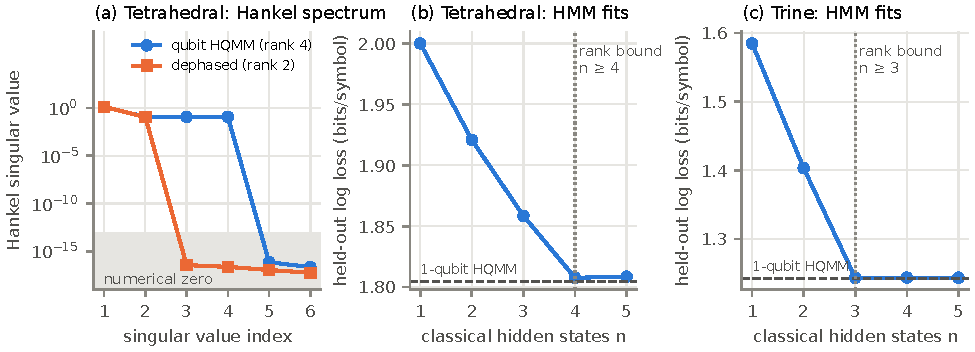
\includegraphics[width=\textwidth]{figures/fig_rank_and_fits.pdf}
  \caption{(a)~Hankel singular values (strings up to length 3) of the tetrahedral qubit model and its computational-basis dephasing; four non-zero values certify that any classical HMM needs four settings. (b,\,c)~Held-out log loss of $n$-setting HMMs fitted by Baum--Welch; dashed: the true one-qubit model; dotted: the rank bound.}
  \label{fig:main}
\end{figure}

\section{Preliminary experiments}\label{sec:experiments}

All numbers come from one script with a fixed random seed (code in \texttt{analysis/}); a second run gave identical results.

\paragraph{Generic quantum models reach the ceiling.} The Hankel rank was 4 for all of 20 random qubit HQMMs (3 symbols, random isometries) and 9 for all of 20 random qutrit HQMMs; their dephased versions had rank 2 and 3. A generic $d$-dimensional quantum memory thus produces a process no HMM with fewer than $d^2$ settings can reproduce; the examples of Section~\ref{sec:example} are simply the ones we can analyse by hand.

\paragraph{Does the bound show up in learning?} The rank bound concerns \emph{exact} reproduction. To test prediction, we sampled 10{,}000 training and 10{,}000 held-out symbols from the tetrahedral and trine models and fitted HMMs with $n=1,\dots,5$ settings by Baum--Welch (expectation--maximisation), 8 random initialisations per $n$. Table~\ref{tab:fits} and Figure~\ref{fig:main}(b,\,c) give the held-out log loss: average bits needed to encode each next symbol (lower is better).

\begin{table}[h]
\centering\footnotesize
\begin{tabular}{lccccc|cc|c}
\toprule
 & \multicolumn{5}{c|}{Classical HMM, $n$ settings} & Best dephased & True & Exact \\
Data from & $n=1$ & 2 & 3 & 4 & 5 & qubit model & 1-qubit model & entropy rate \\
\midrule
Tetrahedral & 2.000 & 1.921 & 1.859 & \textbf{1.808} & 1.809 & 1.921 & 1.804 & 1.792 \\
Trine & 1.585 & 1.403 & \textbf{1.243} & 1.244 & 1.243 & 1.400 & 1.242 & 1.252 \\
\bottomrule
\end{tabular}
\caption{Held-out log loss (bits per symbol). Classical HMMs match the one-qubit model at exactly the size the rank bound requires (bold) and not before. ``Best dephased'' is the best of 156 bases spread over the Bloch sphere.}
\label{tab:fits}
\end{table}

First, the fits reach the quantum model exactly where Lemma~\ref{lem:hankel} allows and not before: with three settings the tetrahedral data cost 0.054 extra bits per symbol, with two 0.116. Second, this is not an optimisation failure: the 8 restarts agree closely (for $n=4$, training losses 1.7935--1.7944), so small models are limited by their size, the distinction our proposal set out to draw. Third, removing coherence is costly: the best dephased qubit model is no better than the best 2-setting HMM, and a bad basis is far worse (for the trine, dephasing perpendicular to the plane of the states gives 1.585 bits, the same as no memory). \emph{Caveat:} held-out estimates carry about $\pm0.01$ bits of sampling noise (the true model scores 1.804 against an exact rate of 1.792); all entries share one test sample, so differences are more reliable than absolute values.

\section{What ``more compact'' does and does not mean (Q3)}\label{sec:resources}

\begin{table}[h]
\centering\footnotesize
\begin{tabular}{lll}
\toprule
Measure & One-qubit HQMM & Smallest classical HMM \\
\midrule
Memory dimension & 2 & 4 (certified) \\
Memory entropy (stationary) & 1 bit ($\rho=I/2$) & 2 bits (last-symbol model) \\
Numbers stored per step, simulated classically & 3 (Bloch vector) & 3 (belief over 4 settings) \\
Free parameters of the model family & 28 & 24 or 60 \\
Prediction quality & exact & exact \\
\bottomrule
\end{tabular}
\caption{Resources for the tetrahedral process (trine: entropy 1 vs.\ $\log_2 3\approx1.585$ bits). The qubit family is an $8\times2$ complex isometry, $32-4=28$ real parameters before symmetries; a 4-setting HMM has 24 if symbols depend only on the current setting, 60 in the transition-emitting form used here.}
\label{tab:resources}
\end{table}

Table~\ref{tab:resources} compares the qubit model with the smallest classical HMM measure by measure. The defensible claim is narrow: a \emph{physical} quantum memory carried between steps can be smaller, in dimension and entropy, than any classical memory producing the same statistics. Several things do not follow.
\begin{itemize}
\item \textbf{No classical speedup or storage saving.} Simulating the qubit model classically means tracking a $2\times2$ density matrix, which costs as much as the 4-setting belief; a $d$-dimensional HQMM is a $d^2$-dimensional linear model.
\item \textbf{The comparison class matters.} Lemma~\ref{lem:hankel} also bounds \emph{signed} linear models (OOMs~\cite{jaeger2000}), and a 4-dimensional OOM reproduces the qubit process exactly. The advantage is over HMMs, whose memory must be a probability distribution.
\item \textbf{The rank bound certifies at most a quadratic gap.} Since an HQMM has $\rank H\le d^2$, the Hankel argument can never show more than $d$ versus $d^2$. Larger gaps, such as the unbounded one-qubit advantage of Elliott \emph{et al.}~\cite{elliott2020}, need a different certificate. The natural classical quantity is the \emph{nonnegative} rank of $H$: the proof of Lemma~\ref{lem:hankel} factorises $H$ into nonnegative matrices with inner dimension $n$, and this rank can exceed the ordinary one.
\item \textbf{Our examples are simple.} In the SIC models the memory just encodes the last symbol in non-orthogonal states. Random HQMMs reach the ceiling without this structure; the final report will test whether the learning results carry over.
\end{itemize}

\section{Plan for the final report and poster}\label{sec:plan}

The final report keeps this structure and adds: (1)~a \textbf{circuit realisation} of each instrument through the isometry $V = \sum_x \ket{x}\otimes K_x$ (one memory qubit and two ancillas for the tetrahedral model), simulated and checked against the sequence probabilities; (2)~a \textbf{published example}, the process of~\cite{ghafari2019} or the synthetic HQMM of~\cite{srinivasan2018}, under the same rank, dephasing and fitting analysis; (3)~how the larger separations of~\cite{elliott2020} are \textbf{certified}, and \textbf{nonnegative-rank} bounds for our examples where feasible; (4)~the fitting experiment on \textbf{random HQMMs}, whose memory does more than store the last symbol. As a \textbf{stretch goal}, the costliest part of the original plan, we will learn HQMMs with the Stiefel-manifold method of~\cite{adhikary2020} and report it only if solid. The poster (December~10) will centre on the tetrahedral example and Figure~\ref{fig:main}.

\begin{multicols}{2}
\renewcommand{\section}[2]{\subsection*{#2}}
\begin{thebibliography}{9}\footnotesize\setlength{\itemsep}{0pt}
\bibitem{aaronson2015} S.~Aaronson, ``Read the fine print,'' \emph{Nature Physics} \textbf{11}, 291--293 (2015).
\bibitem{adhikary2020} S.~Adhikary, S.~Srinivasan, G.~Gordon, B.~Boots, ``Expressiveness and learning of hidden quantum Markov models,'' \emph{AISTATS 2020}, PMLR \textbf{108}, 4151--4161; arXiv:1912.02098.
\bibitem{elliott2020} T.~J.~Elliott, C.~Yang, F.~C.~Binder, A.~J.~P.~Garner, J.~Thompson, M.~Gu, ``Extreme dimensionality reduction with quantum modeling,'' \emph{Phys.\ Rev.\ Lett.} \textbf{125}, 260501 (2020); arXiv:1909.02817.
\bibitem{ghafari2019} F.~Ghafari, N.~Tischler, J.~Thompson, M.~Gu, \emph{et al.}, ``Dimensional quantum memory advantage in the simulation of stochastic processes,'' \emph{Phys.\ Rev.\ X} \textbf{9}, 041013 (2019).
\bibitem{gu2012} M.~Gu, K.~Wiesner, E.~Rieper, V.~Vedral, ``Quantum mechanics can reduce the complexity of classical models,'' \emph{Nature Communications} \textbf{3}, 762 (2012).
\bibitem{jaeger2000} H.~Jaeger, ``Observable operator models for discrete stochastic time series,'' \emph{Neural Computation} \textbf{12}(6), 1371--1398 (2000).
\bibitem{monras2010} A.~Monras, A.~Beige, K.~Wiesner, ``Hidden quantum Markov models and non-adaptive read-out of many-body states,'' \emph{Applied Mathematical and Computational Sciences} \textbf{3}, 93 (2011); arXiv:1002.2337.
\bibitem{srinivasan2018} S.~Srinivasan, G.~Gordon, B.~Boots, ``Learning hidden quantum Markov models,'' \emph{AISTATS 2018}, PMLR \textbf{84}, 1979--1987; arXiv:1710.09016.
\end{thebibliography}
\end{multicols}

\section*{Use of AI tools}

\paragraph{Tool.} Claude (Anthropic; model Claude Opus 5.5), used through Claude Code, an agent that can read our files, write and run code, and search the web. All uses below took place on November 24, 2026.

\paragraph{In the project work.}
\begin{itemize}\sloppy
\item \textbf{Planning.} Claude read the course rubric and our graded proposal (including the grader's feedback) and listed what the interim report still needed: background accessible without prior knowledge of Markov models, a worked example, preliminary results, an outline, and this statement. It recommended treating HQMM learning as a stretch goal.
\item \textbf{Literature checks.} Claude used web search to confirm the bibliographic details and abstract-level claims of all eight references. It read abstracts and summaries, not the full papers; statements in this report about those papers rest on that level of reading, and we will check them against the full texts for the final report.
\item \textbf{Code and numbers.} Claude wrote all the analysis code (\texttt{analysis/hqmm.py}: HMM and HQMM models in a common linear form, Hankel matrices, dephasing, sampling; \texttt{analysis/em.py}: Baum--Welch with batched restarts; \texttt{analysis/prelim\_experiments.py}: the experiments; \texttt{analysis/make\_figures.py}: Figure~\ref{fig:main}), ran it, and reran it to confirm that the results are reproducible. Every number in Sections~\ref{sec:embedding}--\ref{sec:resources} comes from that code.
\item \textbf{Ideas.} Claude proposed the tetrahedral, trine and qutrit SIC examples, Proposition~\ref{prop:coherence} and its proof, the use of the Hankel rank as the classical lower bound (Lemma~\ref{lem:hankel}) together with its quadratic ceiling, the basis scan for dephasing, and the resource comparison in Table~\ref{tab:resources}.
\end{itemize}

\paragraph{In writing this report.} Claude drafted the full text of this report in \LaTeX{} from its analysis notes, including the proofs, tables and figure. \groupnote{describe what each of us changed, rewrote or cut in the draft.}

\paragraph{What we verified ourselves.} \groupnote{list what we checked by hand, e.g.\ re-deriving Proposition~1, Lemma~1 and the tetrahedral transition probabilities, reading the code, rerunning the script; and state any AI use in the earlier proposal or elsewhere in the project that is not listed above.} We are responsible for every claim in this report and expect to explain any of it without the tool at the poster session.

\end{document}
